\documentclass[main.tex]{subfiles}

\begin{document}

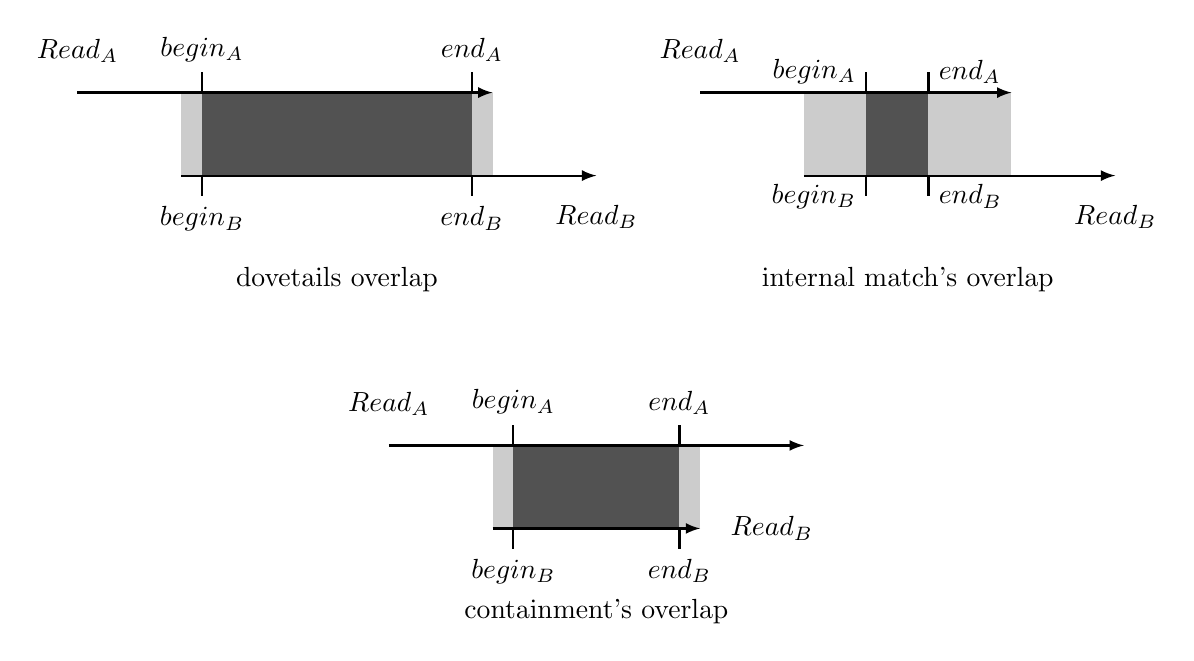
\begin{tikzpicture}[x=0.75pt,y=0.75pt,yscale=-1,xscale=1]

%%%%%%%%%%%%%%%%%%%%%%%%%%%%%%%%%%%%%%%%%%%%%%%%%%%%%%%%%%%%%%%%%%%%%%%%

\draw [fill opacity=1, ->, >=latex, thick, black] (0, 40) -- (200, 40);
\draw (0, 20) node {\texttt{$Read_A$}};

\draw [fill opacity=1, ->, >=latex, thick, black] (50, 80) -- (250, 80);
\draw (250, 100) node {\texttt{$Read_B$}};

\draw [fill=black, opacity=0.2, draw=none] (50, 40) rectangle (200, 80);
\draw [fill=black, opacity=0.6, draw=none] (60, 40) rectangle (190, 80);

\draw [fill opacity=1, thick, black] (60, 40) -- (60, 30) node [above] {$begin_A$};
\draw [fill opacity=1, thick, black] (190, 40) -- (190, 30) node [above] {$end_A$};
\draw [fill opacity=1, thick, black] (60, 80) -- (60, 90) node [below] {$begin_B$};
\draw [fill opacity=1, thick, black] (190, 80) -- (190, 90) node [below] {$end_B$};

\draw (125, 130) node {dovetails overlap};

%%%%%%%%%%%%%%%%%%%%%%%%%%%%%%%%%%%%%%%%%%%%%%%%%%%%%%%%%%%%%%%%%%%%%%%%

\draw [fill opacity=1, ->, >=latex, thick, black] (300, 40) -- (450, 40);
\draw (300, 20) node {\texttt{$Read_A$}};

\draw [fill opacity=1, ->, >=latex, thick, black] (350, 80) -- (500, 80);
\draw (500, 100) node {\texttt{$Read_B$}};

\draw [fill=black, opacity=0.2, draw=none] (350, 40) rectangle (450, 80);
\draw [fill=black, opacity=0.6, draw=none] (380, 40) rectangle (410, 80);

\draw [fill opacity=1, thick, black] (380, 40) -- (380, 30) node [left] {$begin_A$};
\draw [fill opacity=1, thick, black] (410, 40) -- (410, 30) node [right] {$end_A$};
\draw [fill opacity=1, thick, black] (380, 80) -- (380, 90) node [left] {$begin_B$};
\draw [fill opacity=1, thick, black] (410, 80) -- (410, 90) node [right] {$end_B$};

\draw (400, 130) node {internal match's overlap};

%%%%%%%%%%%%%%%%%%%%%%%%%%%%%%%%%%%%%%%%%%%%%%%%%%%%%%%%%%%%%%%%%%%%%%%%

\draw [fill opacity=1, ->, >=latex, thick, black] (150, 210) -- (350, 210);
\draw (150, 190) node {\texttt{$Read_A$}};

\draw [fill opacity=1, ->, >=latex, thick, black] (200, 250) -- (300, 250);
\draw (310, 250) node [right] {\texttt{$Read_B$}};

\draw [fill=black, opacity=0.2, draw=none] (200, 210) rectangle (300, 250);
\draw [fill=black, opacity=0.6, draw=none] (210, 210) rectangle (290, 250);

\draw [fill opacity=1, thick, black] (210, 210) -- (210, 200) node [above] {$begin_A$};
\draw [fill opacity=1, thick, black] (290, 210) -- (290, 200) node [above] {$end_A$};
\draw [fill opacity=1, thick, black] (210, 250) -- (210, 260) node [below] {$begin_B$};
\draw [fill opacity=1, thick, black] (290, 250) -- (290, 260) node [below] {$end_B$};

\draw (250, 290) node {containment's overlap};

%%%%%%%%%%%%%%%%%%%%%%%%%%%%%%%%%%%%%%%%%%%%%%%%%%%%%%%%%%%%%%%%%%%%%%%%

\end{tikzpicture}

\end{document}
